\documentclass[12pt,a4paper]{article}

\usepackage[utf8]{inputenc}
\usepackage[T1]{fontenc}
\usepackage{babel}
\babelprovide[main,import]{spanish}
\usepackage[a4paper,margin=2.5cm]{geometry}
\usepackage{lmodern}
\usepackage{microtype}
\usepackage{amsmath}
\usepackage{booktabs}
\usepackage{longtable}
\usepackage{array}
\usepackage{enumitem}
\usepackage{tabularx}
\usepackage{graphicx}
\usepackage{tikz}
\usetikzlibrary{positioning}
\usepackage{eso-pic}
\usepackage{listings}
\usepackage{xcolor}
\usepackage{hyperref}
\usepackage{fancyhdr}
\usepackage{lastpage}

\definecolor{azuluh}{HTML}{123B63}
\definecolor{azulclaro}{HTML}{EAF2F8}
\definecolor{gris}{HTML}{5B6573}
\definecolor{naranja}{HTML}{B86B1B}
\lstset{basicstyle=\ttfamily\scriptsize,breaklines=true,breakatwhitespace=false,columns=fullflexible,frame=single,keepspaces=true,showstringspaces=false,literate={á}{{\'a}}1 {Á}{{\'A}}1 {í}{{\'i}}1 {Í}{{\'I}}1 {ó}{{\'o}}1 {Ó}{{\'O}}1 {️}{}1 {📄}{[PDF]}5 {🖼}{[IMG]}5}

\hypersetup{colorlinks=true,linkcolor=azuluh,urlcolor=azuluh,pdftitle={Diseño de la base de datos - Rutas de reparto},pdfauthor={Equipo Digimons}}
\setlength{\parindent}{0pt}
\setlength{\parskip}{6pt}
\renewcommand{\arraystretch}{1.2}
\setlist[itemize]{leftmargin=*,itemsep=2pt}
\setlist[enumerate]{leftmargin=*,itemsep=4pt}
\pagestyle{fancy}
\setlength{\headheight}{15pt}
\fancyhf{}
\lhead{Bases de Datos II}
\rhead{Diseño de la base de datos}
\cfoot{\thepage\ de \pageref{LastPage}}
\renewcommand{\headrulewidth}{0.4pt}

\newcolumntype{Y}{>{\raggedright\arraybackslash}X}
\newcommand{\campo}[1]{\texttt{#1}}
\newcommand{\tabla}[1]{\textsf{\textbf{#1}}}
\newcommand{\dependencia}[2]{\ensuremath{\{\texttt{#1}\}\rightarrow\{\texttt{#2}\}}}
\AddToShipoutPictureBG{%
	\begin{tikzpicture}[remember picture,overlay]
		\node[opacity=0.08] at (current page.center) {
\includegraphics[width=0.72\paperwidth]{../MATCOM.png}};
	\end{tikzpicture}%
}

\begin{document}

\begin{titlepage}
\thispagestyle{empty}
\begin{center}
\vspace*{1cm}
{\Large \textbf{UNIVERSIDAD DE LA HABANA}}\\[0.35cm]
{\large Facultad de Matemática y Computación}\\[1.6cm]
{\Large \textbf{BASES DE DATOS II}}\\[1.5cm]
{\rule{\textwidth}{1pt}}\\[0.5cm]
{\huge \textbf{Informe: Diseño de la base de datos}}\\[0.45cm]
{\Large Gestión para la Generación Automática de Rutas de Reparto}\\[0.5cm]
{\rule{\textwidth}{1pt}}\\[2cm]
\begin{tabular}{ll}
\textbf{Curso:} & 2026--2027 \\
\textbf{Equipo:} & Digimons
\end{tabular}
\vfill
\begin{tabular}{>{\raggedright\arraybackslash}p{6.6cm}c p{3.1cm} p{3.7cm}}
\toprule
\textbf{Integrante} & \textbf{Grupo} & \textbf{Telegram} & \textbf{GitHub}\\
\midrule
Karla Díaz Saura & C312 & @kdiazsr & Krli01\\
Manuel Enrique Cardoso Martínez & C312 & @ManuEC04 & ManuEC04\\
Leonardo Peláez Ascención & C312 & @leosoyyoxd & Brand-Leo\\
Jorge Luis Herrera Cecilia & C312 & @Jorge\_Lhc & Jorge-Luis-Herrera\\
José Alejandro Albanés Febles & C311 & @cuban\_developer & JoseAlejandro0508\\
\bottomrule
\end{tabular}
\vfill
\textit{Informe elaborado conforme a las Orientaciones Metodológicas de Bases de Datos II.}
\end{center}
\end{titlepage}

\tableofcontents
\newpage

\section{Título del proyecto}
\textbf{Gestión para la Generación Automática de Rutas de Reparto.}

\section{Análisis y reformulación de requerimientos}

\subsection{Descripción general}
El proyecto nace de una necesidad muy concreta: organizar mejor una operación de reparto en la que intervienen pedidos, centros, zonas, coordinadores, supervisores y repartidores. La aplicación web permitirá registrar pedidos y paradas, organizar la cobertura territorial, generar rutas, validar la planificación, ejecutar las entregas y analizar sus resultados. La base de datos acompañará todo ese recorrido, de modo que cada decisión pueda rastrearse desde el ingreso del pedido hasta la entrega o su reprogramación.

La solución combina un modelo relacional para la información transaccional con un motor de grafos externo para la red dinámica de vías y puntos de tránsito. Esta separación permite consultar y recorrer eficientemente rutas alternativas sin introducir en el esquema relacional una estructura que cambia y se navega constantemente.

\subsection{Actores y responsabilidades}
\begin{longtable}{p{0.32\textwidth}p{0.62\textwidth}}
\toprule
\textbf{Actor} & \textbf{Responsabilidades principales}\\
\midrule
Administrador & Gestionar usuarios y parámetros generales; impedir pedidos duplicados y asignaciones incompatibles de rutas.\\
Coordinador logístico & Registrar y clasificar pedidos, operar en centros autorizados, seleccionar cargas, generar rutas y resolver reprogramaciones asignadas.\\
Supervisor de operaciones & Revisar rutas, aprobarlas, rechazarlas o solicitar modificaciones, dejando constancia de sus observaciones.\\
Repartidor & Consultar su ruta, ejecutar las paradas, registrar entregas e incidencias y solicitar reprogramaciones.\\
\bottomrule
\end{longtable}

\subsection{Requerimientos funcionales reformulados}
\begin{enumerate}
\item \textbf{Autenticación y autorización.} El sistema centralizará la identidad de los usuarios y aplicará permisos según cuatro roles: administrador, coordinador logístico, supervisor de operaciones y repartidor. La jerarquía será total y disjunta: todo usuario operativo pertenece a un subtipo y no pertenece simultáneamente a dos subtipos incompatibles.
\item \textbf{Gestión de centros, zonas y paradas.} Se registrarán centros de distribución, sus zonas cubiertas y las paradas de destino. Un centro puede cubrir varias zonas y una zona puede ser atendida por varios centros.
\item \textbf{Registro de pedidos.} Un coordinador autorizado ingresará cada pedido, indicando descripción, tipo de entrega (paquetería, documentos o perecederos), prioridad (baja, media o urgente), centro de origen y parada de destino.
\item \textbf{Generación automática de rutas.} El sistema seleccionará pedidos y generará una ruta considerando capacidad del vehículo, distribución territorial, tipos de entrega, prioridad y criterios de equilibrio. La parametrización utilizada quedará almacenada junto a la ruta.
\item \textbf{Supervisión.} Toda ruta propuesta podrá ser revisada por un supervisor. El resultado de la revisión, la fecha y las observaciones se conservarán para auditoría.
\item \textbf{Asignación y ejecución.} Una ruta aprobada podrá asignarse a un repartidor habilitado para el centro correspondiente. El sistema impedirá que tenga dos rutas activas incompatibles.
\item \textbf{Entregas y reprogramaciones.} El repartidor registrará el resultado de cada entrega y sus observaciones. Si falla, podrá crear una solicitud de reprogramación y designar el coordinador que la resolverá; se conservará el resultado manual.
\item \textbf{Reportes y exportación.} Todos los usuarios podrán consultar resultados tabulares y gráficos, ordenar columnas y exportar la información a PDF.
\end{enumerate}

\subsection{Requerimientos informacionales}
La base de datos deberá soportar, como mínimo, las siguientes consultas:
\begin{enumerate}
\item Rutas generadas para un centro, con creador, fecha de creación y parámetros.
\item Pedidos más gestionados en rutas finales, clasificados por prioridad y zona.
\item Rutas validadas por un supervisor, con fecha y observaciones.
\item Desempeño de repartidores en una ruta, agrupado por prioridad y tasa de entrega a tiempo.
\item Comparación de rutas de varios centros por zona, prioridad y cumplimiento de criterios.
\item Correlación entre prioridad y rendimiento por centro; identificación de los diez pedidos con mayor incumplimiento, su coordinador y centro; y comparación entre repartidores que solicitaron reprogramación y el promedio de entrega a tiempo de sus flotas.
\end{enumerate}

\subsection{Requerimientos no funcionales}
\begin{itemize}
\item \textbf{Rendimiento y concurrencia:} las consultas frecuentes sobre disponibilidad y entregas deben responder con baja latencia aun con varios coordinadores conectados.
\item \textbf{Disponibilidad:} el estado de repartidores y paradas en curso debe reflejarse oportunamente durante la jornada.
\item \textbf{Escalabilidad y mantenibilidad:} la arquitectura debe estar desacoplada, documentada, modular y preparada para incorporar nuevas funcionalidades.
\item \textbf{Multiplataforma:} la aplicación web debe poder utilizarse desde los entornos previstos para el equipo y los usuarios.
\item \textbf{Calidad del desarrollo:} se exige control de versiones, planificación, documentación del código, al menos dos patrones de diseño y pruebas unitarias de backend y frontend.
\item \textbf{Red territorial:} la red de conexiones se gestionará independientemente mediante una estructura de grafos adecuada a recorridos y búsquedas dinámicas.
\end{itemize}

\section{Stack tecnológico y arquitectura propuesta}

\subsection{Stack tecnológico}
La solución se implementará como una aplicación web multiplataforma organizada en servicios desacoplados. La selección tecnológica responde a la necesidad de construir una interfaz mantenible, una API con validación estricta, un modelo relacional transaccional y un componente especializado para la red dinámica de vías.

\begin{longtable}{p{0.25\textwidth}p{0.28\textwidth}p{0.39\textwidth}}
\toprule
\textbf{Capa} & \textbf{Tecnologías} & \textbf{Responsabilidad}\\
\midrule
Presentación & React, TypeScript, Vite, React Router & Interfaz web, navegación, formularios, consulta de rutas y visualización de reportes.\\
Estado y datos & TanStack Query & Consumo de la API, caché, sincronización y estados de carga o error.\\
Visualización & Recharts & Gráficos de prioridades, cumplimiento, desempeño y comparación de centros.\\
Backend & Python, FastAPI, Pydantic & API REST, validación de datos, autenticación y coordinación de los casos de uso.\\
Persistencia relacional & PostgreSQL, SQLAlchemy, Alembic & Usuarios, pedidos, centros, rutas, entregas, reprogramaciones y restricciones de integridad.\\
Persistencia de grafos & Neo4j & Zonas, vías, puntos de tránsito, distancias, tiempos estimados y trayectos alternativos.\\
Pruebas & Pytest, Vitest, React Testing Library & Pruebas unitarias del backend y frontend, además de validación de reglas críticas.\\
Ejecución & Docker Compose & Entorno reproducible para frontend, backend, PostgreSQL y Neo4j.\\
Colaboración & GitHub, GitHub Projects, GitHub Actions & Control de versiones, planificación, revisión y ejecución automatizada de pruebas.\\
\bottomrule
\end{longtable}

\subsection{Arquitectura y comunicación}
La arquitectura seguirá un enfoque por capas. React se comunicará con FastAPI mediante una API REST sobre HTTPS. FastAPI separará las rutas HTTP, los servicios de aplicación, los repositorios y las integraciones con PostgreSQL y Neo4j. PostgreSQL será la fuente de verdad para las operaciones transaccionales; Neo4j se utilizará para recorrer la red territorial y sugerir trayectos alternativos. La comunicación entre ambos almacenes se coordinará desde la capa de servicios y no desde la interfaz de usuario.

\begin{itemize}
\item \textbf{Capa de presentación:} componentes React tipados con TypeScript, formularios con validación y vistas de operación y reportes.
\item \textbf{Capa de API:} endpoints REST versionados, esquemas Pydantic y control uniforme de errores.
\item \textbf{Capa de aplicación:} casos de uso para registrar pedidos, generar rutas, validar rutas, registrar entregas y resolver reprogramaciones.
\item \textbf{Capa de persistencia:} repositorios separados para PostgreSQL y Neo4j, con transacciones relacionales y consultas de grafos especializadas.
\item \textbf{Capa de seguridad:} autenticación mediante tokens de acceso y renovación, contraseñas protegidas con Argon2 y autorización según rol y centro habilitado.
\end{itemize}

\subsection{Patrones, calidad y operación}
Se aplicarán el patrón \textbf{Repository} para aislar el acceso a datos, \textbf{Service Layer} para concentrar las reglas de negocio y \textbf{Strategy} para permitir nuevos criterios de equilibrio sin modificar el flujo general de generación de rutas. El código se organizará por responsabilidades, con nombres descriptivos, documentación de funciones públicas y validaciones en los límites de cada servicio.

Las pruebas unitarias cubrirán como mínimo la autorización por rol, la prevención de pedidos duplicados, la asignación exclusiva de repartidores, la generación según criterios, el registro de entregas y la creación de reprogramaciones. El frontend se probará con Vitest y React Testing Library; el backend, con Pytest. GitHub Actions ejecutará estas pruebas automáticamente ante cambios relevantes.

La configuración se gestionará mediante variables de entorno y un archivo de ejemplo. Docker Compose permitirá levantar los servicios de forma reproducible. El repositorio deberá incluir el fichero de dependencias, el archivo `.gitignore`, los servicios necesarios para el entorno local y una planificación visible en GitHub Projects con tareas, responsables, estados, fechas y milestones.

\section{Modelo Conceptual Relacional Extendido (MERX)}

\subsection{Vista conceptual}
El MERX se organiza alrededor de la entidad raíz \textbf{USUARIO} y una especialización ISA total y disjunta en COORDINADOR\_LOGISTICO, REPARTIDOR, SUPERVISOR\_OPERACIONES y ADMINISTRADOR. Las entidades territoriales y operativas se conectan mediante relaciones con cardinalidades explícitas. Los atributos propios de las relaciones N:M se representan como atributos de \textbf{RUTA\_PARADA} y \textbf{RUTA\_CRITERIO} en el esquema relacional.

\begin{figure}[htbp]
\centering
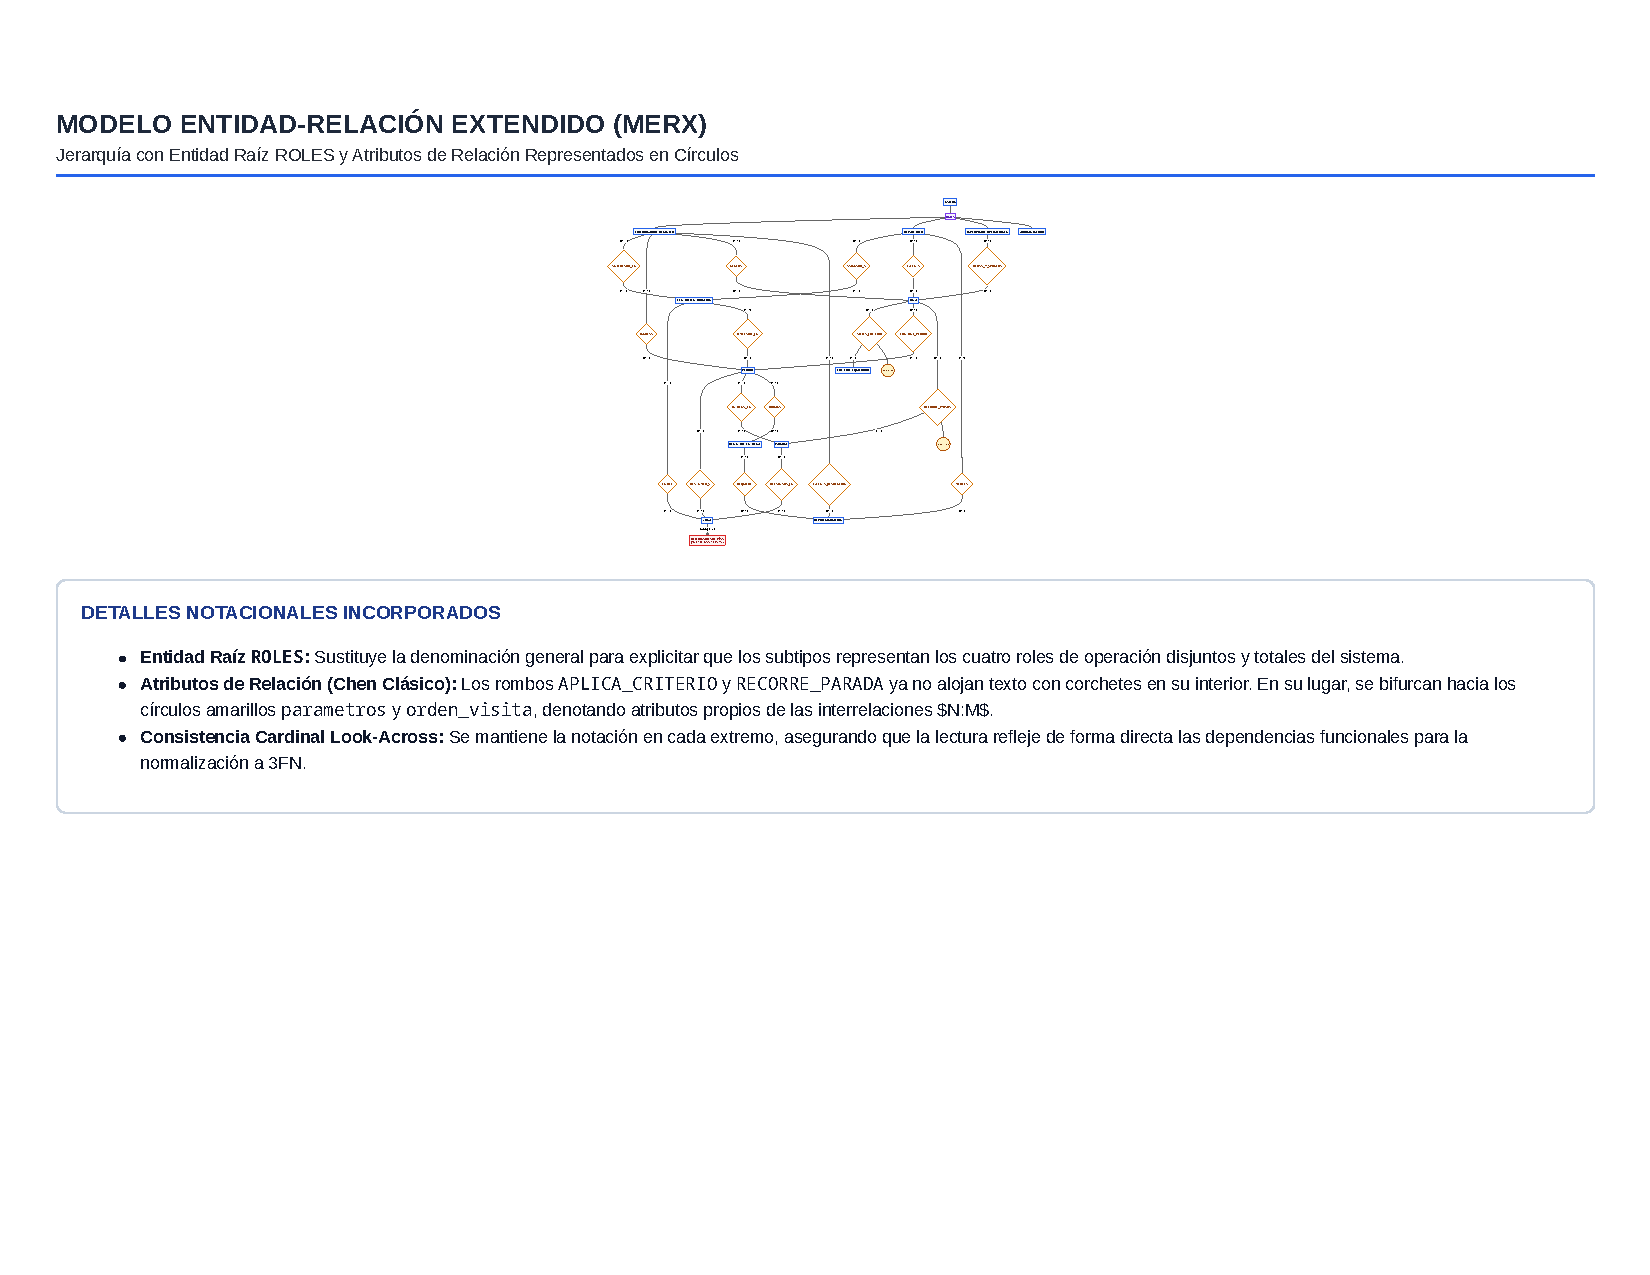
\includegraphics[width=\textwidth,height=0.58\textheight,keepaspectratio]{../MERX.pdf}
\caption{Modelo Entidad-Relación Extendido (MERX).}
\label{fig:merx}
\end{figure}

\subsection{Entidades y relaciones principales}
\begin{itemize}
\item \textbf{Usuarios y roles:} USUARIO centraliza nombre, correo, credenciales, estado y renovación de sesión. Cada subtipo agrega sus atributos específicos.
\item \textbf{Territorio:} CENTRO\_DISTRIBUCION se relaciona con ZONA mediante CUBRE; PARADA se localiza en una zona. La topología vial queda fuera del modelo relacional.
\item \textbf{Carga:} PEDIDO es ingresado por un coordinador, radicado en un centro y destinado a una parada. Una ruta contiene cero o más pedidos seleccionados, resolviendo la trampa de conexión entre planificación y ejecución.
\item \textbf{Planificación:} RUTA es generada por un coordinador, se origina en un centro, puede ser validada por un supervisor y ejecutada por un repartidor. RUTA\_PARADA conserva el orden de visita y RUTA\_CRITERIO conserva la parametrización aplicada.
\item \textbf{Trazabilidad:} cada REGISTRO\_ENTREGA documenta un pedido; una entrega fallida puede originar una REPROGRAMACION solicitada por el repartidor y resuelta por un coordinador.
\end{itemize}

\section{Especificación de restricciones de integridad}

\subsection{Integridad de entidad}
Toda tabla posee una clave primaria no nula y única. Las claves principales son `id\_usuario`, `id\_coordinador`, `id\_repartidor`, `id\_supervisor`, `id\_admin`, `id\_centro`, `id\_zona`, `id\_parada`, `id\_pedido`, `id\_criterio`, `id\_ruta`, `id\_entrega` e `id\_reprogramacion`. Las tablas asociativas utilizan claves compuestas: `(id\_centro,id\_zona)`, `(id\_ruta,id\_parada)`, `(id\_ruta,id\_criterio)`, entre otras.

\subsection{Integridad referencial}
\begin{itemize}
\item Cada subtipo de usuario referencia exactamente un USUARIO existente.
\item PEDIDO referencia un coordinador, centro y parada existentes; la ruta es nullable mientras el pedido no haya sido despachado.
\item PARADA referencia una ZONA existente. CENTRO\_ZONA relaciona únicamente centros y zonas existentes.
\item RUTA referencia al coordinador que la genera y al centro de origen; supervisor y repartidor pueden ser nulos hasta completar esas etapas.
\item RUTA\_PARADA y RUTA\_CRITERIO solo pueden referenciar rutas, paradas y criterios existentes.
\item REGISTRO\_ENTREGA referencia un PEDIDO existente y REPROGRAMACION referencia una entrega existente.
\end{itemize}

\subsection{Restricciones de negocio}
\begin{enumerate}
\item \textbf{No duplicados:} se definirá una restricción única sobre los atributos que identifiquen el mismo pedido dentro del negocio, además de validación de aplicación.
\item \textbf{Autorización:} un coordinador solo puede registrar pedidos o generar rutas para centros presentes en COORDINADOR\_CENTRO.
\item \textbf{Asignación exclusiva:} un repartidor no puede tener más de una ruta activa incompatible; se garantizará mediante validación transaccional y una restricción de unicidad parcial si el gestor lo permite.
\item \textbf{Consistencia geográfica:} la parada debe pertenecer a una zona válida y la combinación centro-zona debe existir cuando el pedido o ruta se asignen al centro.
\item \textbf{Persistencia de criterios:} los parámetros se almacenan como una instantánea en RUTA\_CRITERIO, de modo que cambios posteriores en el criterio no alteren la trazabilidad histórica.
\item \textbf{Reprogramación válida:} solo una entrega registrada y no completada puede generar una solicitud; el estado y la fecha de resolución deben ser coherentes.
\item \textbf{Estados controlados:} prioridad, tipo de entrega, estado de pedido, estado de ruta y resultado de entrega deben restringirse a dominios definidos por el sistema.
\end{enumerate}

\section{Valoración de la corrección del diseño}

\subsection{Dependencias funcionales y normalización}
A partir del universo de atributos se obtiene el siguiente conjunto representativo de dependencias funcionales:
\begin{align*}
\campo{id\_usuario} &\rightarrow \text{datos generales del usuario},\\
\campo{id\_pedido} &\rightarrow \text{datos del pedido, coordinador, centro y parada},\\
\campo{id\_parada} &\rightarrow \campo{id\_zona},\\
\campo{id\_ruta} &\rightarrow \text{fechas, capacidad, estado, coordinador y centro},\\
(\campo{id\_ruta},\campo{id\_parada}) &\rightarrow \campo{orden\_visita},\\
(\campo{id\_ruta},\campo{id\_criterio}) &\rightarrow \campo{parametros\_configuracion}.
\end{align*}
La dependencia `id\_pedido \textrightarrow id\_zona` no se conserva como dependencia independiente porque se deriva transitivamente de `id\_pedido \textrightarrow id\_parada` y `id\_parada \textrightarrow id\_zona`. El esquema resultante elimina esa redundancia y evita anomalías de actualización.

La síntesis por determinantes produce, entre otras, las tablas USUARIO, los subtipos de rol, CENTRO\_DISTRIBUCION, ZONA, CENTRO\_ZONA, PARADA, PEDIDO, CRITERIO\_EQUILIBRIO, RUTA, RUTA\_PARADA, RUTA\_CRITERIO, COORDINADOR\_CENTRO, REPARTIDOR\_CENTRO, REGISTRO\_ENTREGA y REPROGRAMACION. Cada relación contiene atributos que dependen de su clave, de toda su clave y de ningún atributo no clave; por tanto, satisface 3FN bajo las dependencias declaradas.

\subsection{Preservación y reunión sin pérdida}
Las dependencias se preservan porque cada determinante y sus atributos dependientes aparecen en una relación del esquema sintetizado. Las claves foráneas conservan los vínculos semánticos y permiten reconstruir la información mediante reuniones sin pérdida. La asociación directa RUTA--PEDIDO evita perder la relación entre una expedición y su carga cuando una parada concentra pedidos de distintos recorridos.

\subsection{Decisiones de implementación recomendadas}
\begin{itemize}
\item Usar transacciones para generar rutas, asignar repartidores y registrar entregas.
\item Indexar claves foráneas, estados operativos, fechas, centro y prioridad para soportar los reportes.
\item Aplicar control de concurrencia al consultar disponibilidad y al confirmar asignaciones.
\item Mantener la red vial en el motor de grafos y almacenar en el modelo relacional las referencias necesarias para enlazar paradas y zonas.
\item Implementar una arquitectura desacoplada por capas o módulos, aplicar al menos dos patrones y acompañar backend y frontend con pruebas unitarias.
\end{itemize}

\section{Conclusiones}
Este diseño busca que la base de datos refleje la operación real y no solo una lista de tablas. Los roles representan responsabilidades diferentes; los pedidos conservan su origen, destino y estado; las rutas guardan los criterios con los que fueron generadas; y las entregas permiten saber qué ocurrió en cada parada. Así, la información no se pierde cuando una ruta cambia, una entrega falla o debe solicitarse una reprogramación.

La especialización ISA evita repetir los datos comunes de los usuarios, mientras que las relaciones asociativas permiten representar correctamente las rutas, sus paradas y los criterios aplicados. La red vial se mantiene en un motor de grafos porque sus conexiones y recorridos cambian con mayor frecuencia que los datos administrativos. Esta separación mantiene el modelo relacional claro y deja abierta la posibilidad de buscar alternativas cuando una entrega no puede completarse como estaba prevista.

Las claves, referencias y restricciones de negocio protegen la consistencia de la información; la normalización a 3FN reduce duplicidades y evita anomalías de actualización. Además, el stack tecnológico propuesto permite llevar el modelo a una aplicación mantenible, con una interfaz accesible, una API validada, pruebas automatizadas y un entorno reproducible. El resultado no pretende cerrar todas las decisiones de implementación, pero sí ofrece una base sólida, comprensible y verificable para construir el sistema.

\section*{Fuentes de trabajo utilizadas}
\addcontentsline{toc}{section}{Fuentes de trabajo utilizadas}
\begin{itemize}
\item International Council on Systems Engineering. \textit{Requirements Engineering}, SEBoK v2.14. Disponible en: \url{https://www.sebokwiki.org/wiki/Requirements_Engineering}. Consultado el 9 de octubre de 2026.
\item University of Cape Town. \textit{Chapter 6: Entity-Relationship Modelling}. Material académico de bases de datos. Disponible en: \url{https://www.cs.uct.ac.za/mit_notes/database/htmls/chp06.html}. Consultado el 9 de octubre de 2026.
\item University of Cape Town. \textit{Chapter 7: Enhanced Entity-Relationship Modelling}. Material académico sobre especialización, generalización y restricciones ISA. Disponible en: \url{https://www.cs.uct.ac.za/mit_notes/database/htmls/chp07.html}. Consultado el 9 de octubre de 2026.
\item University of Cape Town. \textit{Chapter 8: Data Normalisation}. Material académico sobre dependencias funcionales y 1FN--3FN. Disponible en: \url{https://www.cs.uct.ac.za/mit_notes/database/htmls/chp08.html}. Consultado el 9 de octubre de 2026.
\item PostgreSQL Global Development Group. \textit{Data Definition and Constraints}. Documentación oficial sobre claves, restricciones e integridad referencial. Disponible en: \url{https://www.postgresql.org/docs/current/ddl-constraints.html}. Consultado el 9 de octubre de 2026.
\item Neo4j, Inc. \textit{Get Started with Neo4j}. Documentación oficial sobre bases de datos de grafos y Cypher. Disponible en: \url{https://neo4j.com/docs/getting-started/current/}. Consultado el 9 de octubre de 2026.
\item React. \textit{React Documentation: Learn}. Documentación oficial sobre componentes y estado de interfaces. Disponible en: \url{https://react.dev/learn}. Consultado el 9 de octubre de 2026.
\item FastAPI. \textit{FastAPI Documentation}. Documentación oficial sobre APIs, validación y OpenAPI. Disponible en: \url{https://fastapi.tiangolo.com/}. Consultado el 9 de octubre de 2026.
\item Docker. \textit{Get Started}. Documentación oficial sobre contenedores y entornos reproducibles. Disponible en: \url{https://docs.docker.com/get-started/}. Consultado el 9 de octubre de 2026.
\item GitHub. \textit{About Projects}. Documentación oficial sobre planificación mediante tableros, milestones y seguimiento de tareas. Disponible en: \url{https://docs.github.com/en/issues/planning-and-tracking-with-projects/learning-about-projects/about-projects}. Consultado el 9 de octubre de 2026.
\end{itemize}

\end{document}
